% ======================================================================
% ISPA 2026 submission draft
% Title: Parallel Mechanism-Aware Multi-Objective Optimization for
%        Post-Disaster Road Recovery and Relief Logistics
% Format: IEEEtran, 10pt, two-column, letterpaper
% Status: FIRST DRAFT -- pilot-scale evidence; parallel experiments in progress
% ======================================================================
\documentclass[10pt,conference,letterpaper]{IEEEtran}

\usepackage[utf8]{inputenc}
\usepackage{amsmath,amssymb}
\usepackage{graphicx}
\usepackage{booktabs}
\usepackage{multirow}
\usepackage{tikz}
\usetikzlibrary{shapes,arrows,positioning,fit}
\usepackage{hyperref}
\hypersetup{hidelinks}

% Compact lists to save space
\usepackage{enumitem}
\setlist[itemize]{nosep,leftmargin=1.2em}
\setlist[enumerate]{nosep,leftmargin=1.4em}

\newcommand{\F}{\mathcal{F}}
\tikzstyle{block} = [rectangle, draw, rounded corners, text centered,
    minimum height=2.0em, minimum width=7.5em, font=\footnotesize]
\tikzstyle{arrow} = [thick,->,>=stealth]

\begin{document}

\title{Parallel Mechanism-Aware Multi-Objective Optimization\\
for Post-Disaster Road Recovery and Relief Logistics}

% TODO(authors): fill in author names, affiliations, and contact emails before submission.
\author{\IEEEauthorblockN{Kai-Kai Li\thanks{Corresponding author.}}
\IEEEauthorblockA{Department of XXX, University of XXX\\
City, Country\\
\texttt{\{email\}@xxx.edu}}
}

\maketitle

\begin{abstract}
Post-disaster road recovery and relief logistics are tightly coupled:
repair scheduling determines when the network becomes traversable, while
delivery decisions determine how much relief reaches demand nodes and when.
Recent models enrich this coupling with complex physical mechanisms---%
progressive recovery (PR), heterogeneous vehicle accessibility thresholds
(HT), and edge-period throughput capacity (EC)---that improve fidelity but
make every candidate solution expensive to evaluate through multi-period
network simulation. This paper studies not only how to optimize such a
realistic recovery--logistics system, but also \emph{when} its complex
mechanisms actually matter and \emph{how} their expensive evaluations can
be efficiently parallelized. We formalize a three-layer mechanism-aware
diagnosis---structural/dynamic exposure, dispatch participation, and
objective effect---that separates mechanisms that merely exist from those
that change dispatch behavior and, ultimately, optimization objectives.
We then present a master--worker parallel multi-objective framework in
which fitness evaluation of the full multi-period simulation is distributed
across workers while selection, crossover, mutation, random-number
generation, archiving, and budget accounting stay centralized, preserving
exact reproducibility of the optimization protocol. Pilot diagnostics on
the Wenchuan WEN38 network and multi-scale synthetic networks (S025, S050,
M100) locate the applicability conditions of PR, HT, and EC, and
micro-benchmarks quantify the wall-clock savings of parallel population
evaluation.
\end{abstract}

\begin{IEEEkeywords}
disaster relief logistics; road network recovery; multi-objective
optimization; NSGA-II; parallel evolutionary computation;
mechanism applicability; progressive recovery.
\end{IEEEkeywords}

% ======================================================================
\section{Introduction}
\label{sec:intro}
% ======================================================================

In the aftermath of a major earthquake, two operations proceed in lockstep:
crews repair damaged roads, and fleets deliver relief supplies over the
recovering network. The two are inseparable---a repair schedule is only as
good as the deliveries it enables, and a delivery plan is only feasible on
the network that repairs make available. Joint optimization of
\emph{road recovery} and \emph{relief logistics} over a multi-period
horizon is therefore the natural formulation, following the line of
Li and Teo~\cite{li2019post}.

Realism comes at a price. Three physical mechanisms substantially improve
model fidelity. \emph{Progressive recovery} (PR) recognizes that a damaged
road is not simply ``broken'' or ``fixed'': it passes through blocked,
temporary, single-lane, and basic stages, each admitting different traffic.
\emph{Heterogeneous vehicle accessibility} (HT) recognizes that a heavy
truck and a light van do not share the same passability threshold on a
partially recovered road. \emph{Edge-period capacity} (EC) recognizes that
each road segment can only carry a bounded throughput per period. Each
mechanism is physically plausible, and each makes the evaluation of a
single candidate solution more expensive: decoding a solution requires a
full multi-period simulation of repair progress, vehicle-specific
passability graphs, capacity-constrained dispatch, and fair allocation.

This raises two gaps that existing work rarely addresses together.
\emph{First}, it is unclear \emph{when} these complex mechanisms genuinely
enter the decision. A mechanism can be present in the model yet never bind:
if no delivery ever uses a partially recovered road, PR changes nothing;
if fleet capacity is ample, EC is vacuous. Optimizing with a full-fidelity
model in a regime where its mechanisms are dormant wastes computation and
obscures which physics actually drives the trade-offs. \emph{Second}, even
where the mechanisms matter, the sheer cost of full-fidelity multi-period
evaluation---repeated for every candidate in every generation of an
evolutionary optimizer---dominates runtime and limits the affordable
search budget, especially as networks grow.

The two gaps are two sides of one coin. Mechanism-aware analysis asks
whether the expensive physics is worth simulating at all in a given
regime; parallel evaluation asks how to afford the simulation where the
answer is yes. Together they reframe the problem: we study not only how
to optimize a realistic post-disaster recovery--logistics system, but
also \emph{when} its complex physical mechanisms matter and \emph{how}
their expensive evaluations can be efficiently parallelized.

This paper proposes a \emph{mechanism-aware parallel} framework that
addresses both gaps. Our contributions are fourfold:

\begin{enumerate}
\item \textbf{A mechanism-aware diagnosis methodology.} We separate three
evidence layers---\emph{structural/dynamic exposure} (a mechanism could
matter), \emph{dispatch participation} (it changes actual dispatches), and
\emph{objective effect} (it changes the optimization objectives)---and
establish their logical relations, including where the chain breaks. This
turns ``does the mechanism matter?'' from parameter sweeping into
verifiable conditions.

\item \textbf{Applicability conditions for PR, HT, and EC.} Pilot
diagnostics on the Wenchuan WEN38 network and multi-scale synthetic
networks locate non-binding, transition, and binding zones for each
mechanism, e.g.\ EC never binds below an edge-utilization of 0.85 and a
sharper rerouting-based criterion, and PR exposure is jointly governed by
repair time, crew count, and period length.

\item \textbf{A master--worker parallel multi-objective optimization
framework.} Population fitness evaluation---the expensive multi-period
simulation---is distributed across parallel workers, while selection,
crossover, mutation, RNG, archiving, and budget accounting remain
centralized. The design guarantees that the optimization protocol is
unchanged: identical seeds yield identical Pareto fronts for any worker
count.

\item \textbf{Empirical validation.} We evaluate along four research
questions covering mechanism effects (RQ1), applicability conditions
(RQ2), runtime reduction without protocol change (RQ3), and scalability
with network size and worker count (RQ4).
\end{enumerate}

The remainder of the paper is organized as follows.
Section~\ref{sec:related} reviews related work.
Section~\ref{sec:formulation} formulates the v2 multi-period
recovery--logistics model with PR/HT/EC and three objectives.
Section~\ref{sec:framework} presents the mechanism-aware parallel
optimization framework.
Section~\ref{sec:experiments} reports the experimental evaluation, and
Section~\ref{sec:conclusion} concludes.

% ======================================================================
\section{Related Work}
\label{sec:related}
% ======================================================================

\paragraph{Post-disaster road recovery and relief logistics.}
The coupling of network repair scheduling with relief distribution has been
studied as multi-period optimization since Li and Teo~\cite{li2019post},
who jointly schedule repair work and relief logistics over a damaged
network. The broader disaster-operations literature~\cite{altay2006or,
caunhye2012optimization} covers facility location, inventory, and vehicle
routing under uncertainty, while road-recovery studies focus on repair
sequencing and crew assignment. Progressive (staged) recovery appears in
several infrastructure-restoration models, heterogeneous fleets are
standard in relief routing, and link-capacity constraints are common in
traffic assignment; however, these mechanisms are usually adopted as fixed
modeling choices rather than as objects of study whose decision relevance
is itself diagnosed.

\paragraph{Multi-objective evolutionary optimization.}
NSGA-II~\cite{deb2002fast} remains the workhorse for multi-objective
combinatorial problems, valued for its elitist non-dominated sorting and
crowding-distance diversity. Performance assessment relies on indicators
such as hypervolume (HV) and inverted generational distance
(IGD)~\cite{zitzler2003performance}. Recent work on disaster logistics
applies NSGA-II and hybrids (e.g., with adaptive large-neighborhood
search) to relief-distribution trade-offs among unmet demand, cost, and
fairness. These studies concentrate on \emph{how to optimize} a given
model, not on \emph{when the model's complex mechanisms change the answer}.

\paragraph{Parallel evolutionary and simulation-based optimization.}
Parallel genetic algorithms are well surveyed~\cite{cantu1998survey,
alba2002parallelism}: the dominant paradigms are master--slave (distributed
fitness evaluation), island models (distributed populations with
migration), and fine-grained diffusion models. For simulation-based
optimization, master--slave parallelization of fitness evaluation is the
natural fit because a single evaluation---here, a full multi-period
network simulation---dominates runtime while the evolutionary operators
themselves are cheap. Existing applications rarely combine this with a
diagnosis of \emph{which} expensive model components are actually
decision-relevant, which is precisely the combination this paper pursues:
mechanism-aware analysis decides what fidelity is worth paying for, and
parallel evaluation reduces the cost of paying for it.

% ======================================================================
\section{Problem Formulation}
\label{sec:formulation}
% ======================================================================

We build on the multi-period road repair and relief logistics model of
Li and Teo~\cite{li2019post}, extended with staged recovery,
vehicle-specific accessibility, and per-period edge throughput. Evaluation
semantics follow our v2 contract: dispatches in each period use
\emph{period-start} road conditions, trips longer than one period do not
count as current-period arrivals, and no global supply--demand ratio caps
per-node allocation.

\subsection{Road network, horizon, and damage}

Let $G=(V,E)$ be an undirected road network. The Wenchuan case (WEN38) has
$|V|=38$ nodes, $|E|=51$ edges, of which $|D|=16$ edges are damaged; 3
nodes are supply depots and 35 are demand nodes, with total supply
$9{,}000$~t against total demand $11{,}288$~t (maximum achievable
satisfaction $\approx 79.73\%$). The planning horizon spans $T=9$ periods
of $\eta=8$~h (72~h total). A set of $K=3$ repair crews restores damaged
edges; each crew works on one edge at a time with a known repair duration.

\subsection{Heterogeneous vehicle fleet}

Four vehicle types differ in payload, fleet size, minimum recovery
progress required for passage, and passenger-car-unit (PCU) footprint
(Table~\ref{tab:fleet}). A vehicle may traverse an edge only if the edge's
recovery progress meets its type-specific threshold, and each vehicle
makes at most one trip per period.

\begin{table}[t]
\centering
\caption{Heterogeneous vehicle fleet (WEN38 calibration).}
\label{tab:fleet}
\begin{tabular}{ccccc}
\toprule
Type & Payload (t) & Fleet size & Min.\ progress & PCU \\
\midrule
1 & 5  & 150 & 0.30 & 1.0 \\
2 & 10 & 110 & 0.50 & 1.5 \\
3 & 15 & 70  & 0.70 & 2.0 \\
4 & 20 & 40  & 0.80 & 2.5 \\
\bottomrule
\end{tabular}
\end{table}

\subsection{PR: progressive recovery}

A damaged edge's recovery progress $p\in[0,1]$ maps to discrete stages
with capacity/speed ratios (Table~\ref{tab:stages}). The binary-recovery
counterpart (used in ablations) admits only $p\in\{0,1\}$.

\begin{table}[t]
\centering
\caption{Progressive recovery stages.}
\label{tab:stages}
\begin{tabular}{ccc}
\toprule
Progress $p$ & Stage & Capacity / speed ratio \\
\midrule
$[0,0.30)$ & blocked   & 0 \\
$[0.30,0.60)$ & temporary & 0.30 \\
$[0.60,0.80)$ & one-lane  & 0.60 \\
$[0.80,1)$ & basic     & 0.80 \\
$1$ & full & 1.00 \\
\bottomrule
\end{tabular}
\end{table}

\subsection{HT: heterogeneous accessibility threshold}

Given edge progress $p$, the passable vehicle set is
$\{k : \theta_k \le p\}$ with thresholds $\theta_k$ from
Table~\ref{tab:fleet}. Disabling HT (ablation) unifies all thresholds to
$0.30$ while keeping payloads, PCU footprints, and trip budgets
heterogeneous.

\subsection{EC: edge-period capacity}

Each edge-period admits bounded throughput measured in PCU:
$\sum \text{trips}\times\mathrm{PCU}_k \le \mathrm{cap}(e,t)$, where
$\mathrm{cap}(e,t)$ scales with the edge's recovery stage. When capacity
is exhausted, dispatch reroutes on the residual-capacity graph. Disabling
EC removes throughput accounting but keeps passability.

\subsection{Decision encoding and simulation}

A candidate solution is a triple $x=(\pi,a,\sigma)$: a repair sequence
$\pi$ over damaged edges, a crew assignment $a$ mapping each crew to its
ordered edge list, and a dispatch priority order $\sigma$ over
supplier--demand pairs. Decoding simulates period by period:

\begin{enumerate}
\item Advance repair progress from crew schedules; derive each edge's
stage and capacity/speed ratio (Table~\ref{tab:stages}).
\item Build vehicle-specific passability graphs from \emph{period-start}
conditions using thresholds $\theta_k$ (HT).
\item Allocate relief by a max-min service-level rule, then allocate
remaining servable demand; each allocation respects remaining supply,
remaining demand, per-type trip budgets, passability, single-trip time
$\le\eta$ (within-period arrival), and edge-period PCU capacity, with
rerouting on the residual-capacity graph when EC binds (EC).
\end{enumerate}

Supply and demand carry over across periods; vehicle spatial positions
and return trips are not tracked beyond the exogenous per-period trip
budget, a coarse discrete-time approximation consistent with the
strategic planning level of the model.

\subsection{Model variants for ablation}

To isolate mechanism effects we define three ablated variants of the
full model. \textbf{No-PR} replaces staged recovery with binary
recovery ($p\in\{0,1\}$), removing all intermediate states.
\textbf{No-HT} unifies all passability thresholds to $0.30$ while keeping
payloads, PCU footprints, and trip budgets heterogeneous, so only the
threshold structure is removed. \textbf{No-EC} drops edge-period
throughput accounting but retains passability. Toggling exactly one
mechanism at a time yields paired comparisons in which any change in
$(F_1,F_2,F_3)$ is attributable to that mechanism alone.

\subsection{Objectives}

We minimize three objectives computed by the shared evaluator
\texttt{evaluate\_capacity\_solution()}:

\begin{align}
F_1 &= \sum_{t=1}^{T}\bigl(1 - s_t\bigr),
  &&\text{cumulative unmet demand (proportion--periods),} \label{eq:f1}\\
F_2 &= T_{\text{travel}} + w_r\,
      \bigl(T_{\text{repair}} + T_{\text{transfer}}\bigr),
  &&\text{transport + repair time (weighted minutes),} \label{eq:f2}\\
F_3 &= -\min_{i} s_i^{\text{final}},
  &&\text{worst-node service fairness,} \label{eq:f3}
\end{align}
where $s_t$ is the total demand satisfaction at the end of period $t$,
$s_i^{\text{final}}$ the final satisfaction of demand node $i$, and
$w_r=0.05$ the default repair-time weight. Objective comparisons use fixed
service resolutions ($10^{-8},10^{-6},10^{-8}$) with quantized comparison
keys so that floating-point noise cannot create spurious Pareto points.

% (to be continued: experiments, conclusion, references)
% ======================================================================
\section{Mechanism-Aware Parallel Optimization Framework}
\label{sec:framework}
% ======================================================================

Our framework has two complementary parts: a \emph{mechanism diagnosis}
that determines when PR/HT/EC genuinely affect decisions, and a
\emph{parallel multi-objective optimizer} that makes full-fidelity
evaluation affordable.

\subsection{Mechanism-aware analysis: from existence to effect}
\label{sec:mechanism}

A common pitfall is to conflate ``the mechanism is in the model'' with
``the mechanism changes the decision.'' We separate three evidence
layers of increasing strength:

\begin{description}[nosep,leftmargin=1.2em]
\item[\textbf{L1 -- Structural/dynamic exposure} (necessary, not
sufficient).] The mechanism \emph{could} matter: e.g., a damaged edge
sits in a partially recovered state on some period-start snapshot (PR),
a period-start progress admits a \emph{proper nonempty subset} of
vehicle types (HT), or an edge's throughput utilization is high (EC).
\item[\textbf{L2 -- Dispatch participation} (stronger).] Toggling the
mechanism off changes the actual dispatch---routes, vehicle types,
tonnages, or trip counts---for a fixed decision.
\item[\textbf{L3 -- Objective effect} (definitional).] Toggling the
mechanism changes the quantized objective vector $(F_1,F_2,F_3)$.
\end{description}

Two logical relations, verified over 360 decision--mechanism pairs across
network scales, govern how these layers may be used.
\emph{Objective $\Rightarrow$ dispatch} holds without exception: if the
objectives changed, the canonical dispatch encoding necessarily changed,
so dispatch comparison is a safe \emph{screening} criterion with no false
negatives. The converse fails: on the 100-node network we observed three
cases where the dispatch changed yet all three objectives were
bit-identical---closing HT made two vehicle types interchangeable in
passability while EC was non-binding, so the dispatcher merely swapped
vehicle labels between identical shipments. Allocation-change is
therefore a \emph{conservative} probe (it over-reports), never the
definition; the definition of ``the mechanism matters'' is always the
objective comparison.

Diagnosis proceeds through three probe families.
\emph{Fixed-decision toggle probes} evaluate a fixed set of decisions
(one SPT-constructed plus random draws) with each mechanism switched on
and off, recording exposure, dispatch, and objective indicators per
decision. \emph{Resource grids} sweep fleet, supply, and capacity-scale
multipliers to locate regimes where each mechanism binds, and
\emph{bottleneck relaxation probes} strictly relax one resource at a time
(fleet $\times2$, supply $\times$1.5, road capacity $\times$2) to attribute
binding resources---a strictly more reliable test than inspecting
leftover supply. Finally, \emph{zone calibration} bisects the capacity
scale per (scenario, seed) so that measured edge utilization lands in
targeted inactive/transition/binding bands, because fixed scales cannot
place different seeds inside a narrow transition band. The resulting
applicability conditions are summarized in
Table~\ref{tab:applicability} and detailed in
Section~\ref{sec:experiments}.

\begin{table}[t]
\centering
\caption{Applicability conditions of PR / HT / EC (pilot diagnostics).}
\label{tab:applicability}
\begin{tabular}{p{0.62\columnwidth}p{0.30\columnwidth}}
\toprule
Condition & Finding \\
\midrule
PR binds only if a damaged edge lies on an \emph{actually used} delivery
path while in a partial-recovery state at period start. & Exposure window
jointly governed by (repair time, crew count, period length); longer
repairs \emph{shrink} exposure under fixed crews. \\
\midrule
HT binds only if some edge's period-start progress admits a proper
nonempty subset of vehicle types on a used path with remaining trips.
A bridge/corridor is \emph{sufficient, not necessary}. & Node-role layout
alone raised participation 2/20 $\to$ 6/20 with zero damaged bridges. \\
\midrule
EC binds only at high edge utilization: $<0.85$ never (0/776 cells across
three scales); 0.85--0.97 transition ($\approx$46\%); $\ge$0.97 binding
($\approx$99\%). Sharper: rerouting occurred $\Rightarrow$ binding
(296/296). & Baseline calibration (utilization 0.010--0.034) is far from
binding; non-effect there is a calibration property, not model failure. \\
\bottomrule
\end{tabular}
\end{table}

In non-binding zones, adding the corresponding mechanism cannot
significantly change solutions---this is an \emph{applicability boundary},
not a failure of the model.

\begin{figure}[t]
\centering
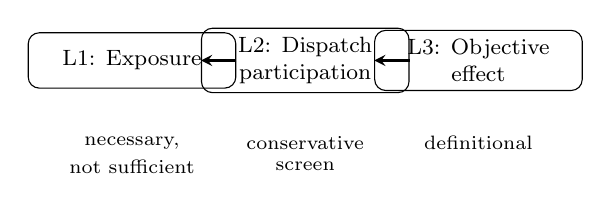
\begin{tikzpicture}[node distance=2.2cm, font=\footnotesize]
\node[block] (l1) {L1: Exposure};
\node[block, align=center, right of=l1] (l2) {L2: Dispatch\\participation};
\node[block, align=center, right of=l2] (l3) {L3: Objective\\effect};
\draw[arrow] (l1) -- (l2);
\draw[arrow] (l2) -- (l3);
\node[font=\scriptsize, below of=l1, yshift=1.15cm] {necessary,};
\node[font=\scriptsize, below of=l1, yshift=0.85cm] {not sufficient};
\node[font=\scriptsize, below of=l2, yshift=1.15cm] {conservative};
\node[font=\scriptsize, below of=l2, yshift=0.85cm] {screen};
\node[font=\scriptsize, below of=l3, yshift=1.15cm] {definitional};
\end{tikzpicture}
\caption{Three-layer mechanism diagnosis. Objective change always implies
dispatch change; the reverse can break (e.g., vehicle-interchange ties),
so L2 screens but never defines.}
\label{fig:diagnosis}
\end{figure}

\subsection{Parallel multi-objective optimization}
\label{sec:parallel}

Even where mechanisms matter, each fitness evaluation runs the full
$T$-period simulation of Section~\ref{sec:formulation}, whose cost grows
with network size. Since candidate evaluations are mutually independent
given the population, we parallelize at the population level with a
master--worker design (Fig.~\ref{fig:framework}).

\begin{figure}[t]
\centering
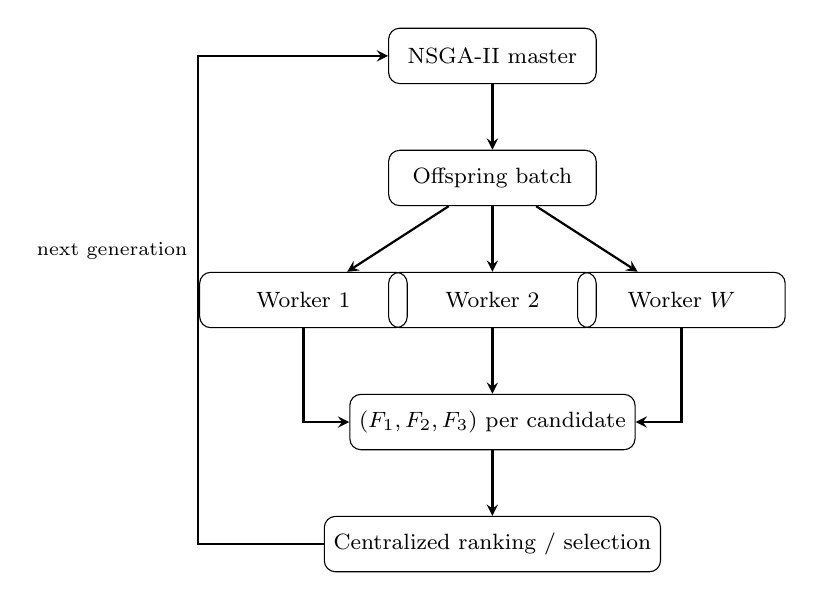
\begin{tikzpicture}[node distance=1.55cm, font=\footnotesize]
\node[block] (nsga) {NSGA-II master};
\node[block, below of=nsga] (batch) {Offspring batch};
\node[block, below of=batch, xshift=-2.4cm] (w1) {Worker 1};
\node[block, below of=batch] (w2) {Worker 2};
\node[block, below of=batch, xshift=2.4cm] (w3) {Worker $W$};
\node[block, below of=w2] (objs) {$(F_1,F_2,F_3)$ per candidate};
\node[block, below of=objs] (sel) {Centralized ranking / selection};
\draw[arrow] (nsga) -- (batch);
\draw[arrow] (batch) -- (w1);
\draw[arrow] (batch) -- (w2);
\draw[arrow] (batch) -- (w3);
\draw[arrow] (w1) |- (objs);
\draw[arrow] (w2) -- (objs);
\draw[arrow] (w3) |- (objs);
\draw[arrow] (objs) -- (sel);
\draw[arrow] (sel.west) -- ++(-1.6cm,0)
  |- node[pos=0.3, left, font=\scriptsize] {next generation} (nsga.west);
\end{tikzpicture}
\caption{Master--worker parallel framework. Only fitness evaluation is
distributed; selection, crossover, mutation, RNG, archiving, and budget
accounting stay centralized, preserving exact reproducibility.}
\label{fig:framework}
\end{figure}

\paragraph{Parallel: fitness evaluation.}
The master generates an offspring batch; each candidate is dispatched to
a worker that runs \texttt{evaluate\_capacity\_solution()} end to end and
returns $(F_1,F_2,F_3)$. Workers are stateless with respect to the search:
they hold no population, no archive, and no RNG state beyond a fixed
evaluation seed.

\paragraph{Centralized: everything else.}
Selection (non-dominated sorting, crowding distance), crossover,
mutation, random-number generation, external archiving, and budget
accounting all remain on the master. The evaluation \emph{budget} counts
evaluations, not generations or wall-clock time, so search effort is
comparable across worker counts.

\paragraph{Reproducibility guarantee.}
Candidates are assigned to workers deterministically and results are
reassembled by candidate index before ranking; all stochasticity flows
from the master's centralized RNG streams. Consequently, identical seeds
produce \emph{bit-identical} evaluated populations---and hence identical
Pareto fronts---for any number of workers $W$. Parallelism changes
\emph{when} results arrive, never \emph{what} the optimizer decides. We
verify this protocol invariance empirically in
Section~\ref{sec:experiments} (RQ3): HV/IGD across $W\in\{1,2,4,8\}$ must
match exactly, while wall-clock time, speedup $S(W)=T_1/T_W$, and
efficiency $E(W)=S(W)/W$ quantify the savings.

This separation is deliberate. Island models exchange migrants and
thereby change the search trajectory; our design keeps the trajectory
fixed and parallelizes only the expensive, independent simulations. The
mechanism-aware analysis of Section~\ref{sec:mechanism} complements it:
it tells us in which zones the full-fidelity evaluation is worth its
cost, while parallelism lowers that cost everywhere.

\begin{figure}[t]
\centering
\begin{minipage}{0.96\columnwidth}
\footnotesize
\textbf{Protocol: master--worker parallel NSGA-II}
\par\smallskip\hrule\par\smallskip
\begin{verbatim}
master(seed):
  rng = init_central_rng(seed)       # all stochasticity here
  P = init_population(rng)
  evaluate_parallel(P)
  archive = nondominated(P)
  repeat until budget exhausted:
    Q = select_crossover_mutate(P, rng)  # centralized
    F = evaluate_parallel(Q)            # distributed
    P = environmental_selection(P,Q)    # centralized
    archive = update(archive, P)
    budget -= |Q|   # budget counts evaluations

evaluate_parallel(C):                # C: candidate batch
  for i, x in enumerate(C):          # deterministic assignment
      send (i, x) to worker (i mod W)
  collect; reassemble results by index i
  return [(F1,F2,F3)] per candidate

worker(i, x):
  return evaluate_capacity_solution(x)
      # full T-period simulation; no search
      # state, no RNG beyond fixed eval seed
\end{verbatim}
\end{minipage}
\caption{Parallel evaluation protocol. Workers are stateless; identical
seeds yield identical Pareto fronts for any worker count $W$.}
\label{fig:protocol}
\end{figure}

\paragraph{Cost structure.}
Each evaluation simulates $T$ periods; per period it rebuilds
vehicle-specific passability graphs (shortest paths over $|E|$ edges)
and runs capacity-constrained, vehicle-aware dispatch over
supplier--demand pairs. The dominant terms therefore grow with network
size and fleet size, while master-side non-dominated sorting costs
$O(MN^2)$ for population $N$ and $M=3$ objectives. The parallelizable
fraction thus approaches one as instances grow, which is exactly where
full-fidelity evaluation hurts most.
% ======================================================================
\section{Experimental Evaluation}
\label{sec:experiments}
% ======================================================================

We structure evaluation around four research questions:

\begin{description}[nosep,leftmargin=1.2em]
\item[\textbf{RQ1.}] Do PR, HT, and EC materially affect
recovery--logistics decisions?
\item[\textbf{RQ2.}] Under what conditions do these mechanisms become
active or binding?
\item[\textbf{RQ3.}] Can parallel evaluation reduce runtime without
changing the optimization protocol?
\item[\textbf{RQ4.}] How does computational scalability change with
network size and worker count?
\end{description}

\paragraph{Instances and protocol.}
We use the Wenchuan WEN38 network and the multi-scale synthetic suite
(S025, S050, M100; M200 in progress): synthetic instances default to a
0.9 supply--demand ratio and capacity scale 0.05, with fleet sized at
0.14$\times$ total demand per period of nominal capacity. The optimizer
is NSGA-II; model-ablation studies use NSGA-II to isolate model effects.
Quality is measured by normalized HV and Euclidean IGD against pooled
reference fronts, with paired main effects, 95\% BCa intervals, and Holm
correction; solver repeats are averaged within an instance before
instances are equally weighted. Ablations toggle one mechanism at a time:
No-PR uses binary recovery, No-HT unifies thresholds to 0.30, and No-EC
drops edge-period throughput. Every saved decision is additionally
replayed under the common Full execution to separate \emph{planning-front
quality}, \emph{selected-solution execution}, and \emph{planning-vs-execution
prediction bias}.

\subsection{RQ1: Do the mechanisms materially affect decisions?}

Pilot ablations show the answer is mechanism- and zone-dependent rather
than a blanket yes. On WEN38, paired small-budget runs find PR
comparisons favoring the Full model, an HT front-quality reversal across
seeds, and zero EC effect at the baseline calibration---consistent with
EC's diagnosed non-binding zone there (Section~\ref{sec:mechanism}).

The cost of ignoring a mechanism is quantified by replaying each
ablated model's planned decisions under the common Full execution
(Table~\ref{tab:replay}, S025 corridor, 813 replayed decisions).
Ignoring EC where it binds underestimates unmet demand by up to 2.73
proportion--periods and misestimates time cost by up to 3{,}783~min, while
in the inactive zone No-EC plans are mathematically identical to Full
(0/93 changed)---exactly the non-binding definition. Ignoring PR changes
most decisions in all zones (33/37, 32/38, 53/58), concentrated in $F_2$
(mean $+$333--1{,}570~min), because one critical road's repair timing
dominates execution cost. Ignoring HT incurs smaller losses (mean
$+$10--115~min in $F_2$). Worst-node fairness ($F_3$) also moves in most
affected decisions, confirming that mechanism effects are not confined
to aggregate objectives.

\begin{table}[t]
\centering
\caption{Cost of ignoring a mechanism: ablated-model decisions replayed
under common Full execution (S025 corridor pilot).}
\label{tab:replay}
\begin{tabular}{llrrrr}
\toprule
Zone & Plan model & \#dec. & Changed & Mean $\Delta F_1$ & Max $|\Delta F_2|$ (min) \\
\midrule
\multirow{3}{*}{inactive}
 & No-PR & 37 & 33 & $-0.798$ & 2{,}663 \\
 & No-HT & 59 & 55 & $+0.275$ & 934 \\
 & No-EC & 93 & \textbf{0} & $0.000$ & 0 \\
\midrule
\multirow{3}{*}{transition}
 & No-PR & 38 & 32 & $-0.166$ & 1{,}039 \\
 & No-HT & 53 & 33 & $+0.129$ & 295 \\
 & No-EC & 93 & 49 & $+0.457$ & 3{,}659 \\
\midrule
\multirow{3}{*}{binding}
 & No-PR & 58 & 53 & $-0.309$ & 745 \\
 & No-HT & 67 & 55 & $+0.034$ & 302 \\
 & No-EC & 93 & \textbf{93} & $+0.691$ & 3{,}783 \\
\bottomrule
\end{tabular}
\end{table}

\subsection{RQ2: When do the mechanisms become active or binding?}

\paragraph{EC: utilization bands with a sharper rerouting criterion.}
Across 1{,}120 grid cells (three scales, two topology families), EC never
alters objectives below 0.85 maximum edge utilization (0/776), binds in
about half the 0.85--0.97 transition cells (22/48), and binds in
$\approx$99\% of cells at $\ge$0.97 (292/296); see
Table~\ref{tab:ecbands}. A sharper sufficient
criterion is \emph{capacity-induced rerouting}: cells with reroutes bind
in 296/296 cases. The 0.97 edge is not a hard threshold (four M100 cells
above it do not bind), so zone selection must calibrate by measured
utilization rather than fixed scales.

\begin{table}[t]
\centering
\caption{EC binding vs.\ maximum edge utilization (1{,}120 cells;
S025/S050/M100).}
\label{tab:ecbands}
\begin{tabular}{lrrrr}
\toprule
Max utilization & S025 & S050 & M100 & Combined \\
\midrule
$<0.85$ & 0/517 & 0/151 & 0/108 & \textbf{0/776} \\
0.85--0.97 & 17/35 & 5/10 & 0/3 & 22/48 (46\%) \\
$\ge$0.97 & 88/88 & 79/79 & 125/129 & 292/296 (99\%) \\
\midrule
\multicolumn{5}{l}{\emph{Rerouting criterion (all scales):}} \\
reroutes $>0$ & \multicolumn{4}{c}{296/296 (100\%)} \\
reroutes $=0$ & \multicolumn{4}{c}{18/824 (2\%)} \\
\bottomrule
\end{tabular}
\end{table}

\paragraph{PR: exposure window governed by crew resources.}
PR exposure requires a damaged edge on an actually used path in a partial
state at period start. Counter-intuitively, under a fixed crew count and
72~h horizon, lengthening repair times \emph{reduces} exposure---more
roads never leave the blocked stage---so the window is jointly controlled
by (repair time, crew count, period length), not by duration alone.

\paragraph{HT: corridor sufficient, not necessary.}
HT needs a used edge whose period-start progress admits a proper nonempty
subset of vehicle types. A damaged bridge is one sufficient topology, but
node-role layout alone raised HT participation from 2/20 to 6/20 with zero
damaged bridges. On the real WEN38 topology with semi-realistic overlays,
a four-level funnel confirms a complete chain: 15/16 damaged edges are
structurally relevant, 5--21 edge--periods per decision show dynamic
exposure, and 19/20 decisions change both dispatch and objectives when HT
is toggled.

\paragraph{Resource bottlenecks.}
Relaxation probes (fleet $\times$2, supply $\times$1.5, road capacity
$\times$2, each strictly a relaxation) show the fleet binds in both
scenario families, with supply co-binding under random damage---there is
no single bottleneck, and ``all supply delivered'' alone cannot identify
one.

\subsection{RQ3: Parallel runtime reduction without protocol change}

We verify two claims: (i)~\emph{protocol invariance}---identical seeds
yield identical fronts for $W\in\{1,2,4,8\}$; and (ii)~\emph{wall-clock
savings}---speedup $S(W)$ and efficiency $E(W)$ of population evaluation.
Table~\ref{tab:parallel} reports a pilot micro-benchmark on the real
v2 evaluator (256 random candidates, WEN38, \texttt{ProcessPoolExecutor}):
objectives are bit-identical across all worker counts, confirming the
reproducibility guarantee of Fig.~\ref{fig:protocol}. Speedup at this
granularity is modest---per-evaluation cost is only $\approx$70~ms, so
process-spawn and IPC overhead dominate---with the best observed mean
speedup of 1.51$\times$ at $W{=}8$ on a 2-core shared VM (so $W{=}4/8$
oversubscribe the cores; a typical 2-worker speedup is
$\approx$1.0--1.35$\times$ with visible run-to-run variance from CPU
contention). Scaling is expected to improve with larger per-dispatch
batches, persistent worker pools, more cores, and larger networks
(M100/M200), where per-evaluation simulation cost dominates;
full-budget NSGA-II measurements are in progress.

\begin{table}[t]
\centering
\caption{Parallel population-evaluation pilot: 256 random candidates on
WEN38 (v2), wall-clock mean of 2 runs on a 2-core shared VM.}
\label{tab:parallel}
\begin{tabular}{ccccc}
\toprule
Workers & Wall-clock (s) & Speedup & Efficiency & Identical objs. \\
\midrule
serial & 18.03 & 1.00 & --- & --- \\
1 & 20.29 & 0.89 & 0.89 & yes \\
2 & 16.10 & 1.12 & 0.56 & yes \\
4 & 16.87 & 1.07 & 0.27 & yes \\
8 & 11.92 & 1.51 & 0.19 & yes \\
\bottomrule
\end{tabular}
\end{table}

The design expectation is near-linear speedup for small $W$ with
efficiency decaying as dispatch/collection overhead and load imbalance
across heterogeneous evaluation times grow; because the master performs
no simulation work, Amdahl's serial fraction is confined to sorting,
selection, and IPC. Critically, any deviation in HV/IGD across $W$ would
indicate a protocol leak (e.g., worker-dependent RNG); none is permitted
by construction. The verification protocol is therefore two-staged:
first assert bit-identical objective vectors for a fixed candidate set
across all $W$ (catching nondeterminism before it can contaminate
search), then compare full NSGA-II runs by HV/IGD against the pooled
reference front together with wall-clock statistics over repeated trials.

\subsection{RQ4: Scalability with network size and worker count}

Per-evaluation cost grows with network size (passability graphs and
capacity-constrained dispatch scale with $|E|$ and the fleet), so the
parallelizable fraction \emph{increases} on larger instances---parallel
evaluation pays off more on M100/M200 than on S025. We report wall-clock
time, speedup, and efficiency across the instance scale ladder for each
$W$, together with per-evaluation timings that decompose simulation cost
vs.\ framework overhead. The mechanism-aware lens adds a second scaling
dimension: in diagnosed non-binding zones, a reduced-fidelity evaluation
(ablated mechanism) can be substituted to cut per-evaluation cost at zero
decision cost, compounding the parallel gains---a direction we leave for
extended experiments.

\paragraph{Validity and limits.}
Current RQ1/RQ2 evidence is pilot-scale (small search budgets, limited
fixed decisions); formal multi-instance, multi-seed statistics with frozen
protocols are the next step before any significance claims. Stress
multipliers are diagnostic, not calibrated field parameters. The parallel
speedups are pilot harness measurements on 256 candidates; full-budget
NSGA-II confirmation across the scale ladder is pending.

% ======================================================================
\section{Conclusion}
\label{sec:conclusion}
% ======================================================================

We studied not only how to optimize a realistic post-disaster
recovery--logistics system, but also when its complex physical mechanisms
matter and how their expensive evaluations can be efficiently
parallelized. Three findings summarize the paper: (1)~complex mechanisms
are not always binding---PR, HT, and EC each have identifiable
non-binding, transition, and binding zones; (2)~mechanism applicability
conditions explain \emph{when} the full model is worth its cost, turning
fidelity selection from guesswork into verifiable conditions; and
(3)~master--worker parallel evaluation reduces the wall-clock cost of
expensive multi-period fitness evaluation without changing the
optimization protocol, with exact reproducibility across worker counts.
Future work includes distributed execution beyond a single node,
larger-scale networks, fidelity-adaptive evaluation driven by the
diagnosed zones, and dynamic rolling-horizon optimization under
revealed repair progress.

% ======================================================================
\begin{thebibliography}{9}
% ======================================================================

\bibitem{li2019post}
S.~Li and K.~L.~Teo, ``Post-disaster multi-period road network repair:
work scheduling and relief logistics optimization,''
\emph{Annals of Operations Research}, vol.~283, pp.~1345--1385, 2019.

\bibitem{deb2002fast}
K.~Deb, A.~Pratap, S.~Agarwal, and T.~Meyarivan, ``A fast and elitist
multiobjective genetic algorithm: NSGA-II,''
\emph{IEEE Trans.\ Evolutionary Computation}, vol.~6, no.~2,
pp.~182--197, 2002.

\bibitem{zitzler2003performance}
E.~Zitzler, L.~Thiele, M.~Laumanns, C.~M.~Fonseca, and V.~G.~da~Fonseca,
``Performance assessment of multiobjective optimizers: an analysis and
review,''
\emph{IEEE Trans.\ Evolutionary Computation}, vol.~7, no.~2,
pp.~117--132, 2003.

\bibitem{cantu1998survey}
E.~Cant{\'u}-Paz, ``A survey of parallel genetic algorithms,''
\emph{Calculateurs Parall{\`e}les, R{\'e}seaux et Syst{\`e}mes
R{\'e}partis}, vol.~10, no.~2, pp.~141--171, 1998.

\bibitem{alba2002parallelism}
E.~Alba and M.~Tomassini, ``Parallelism and evolutionary algorithms,''
\emph{IEEE Trans.\ Evolutionary Computation}, vol.~6, no.~5,
pp.~443--462, 2002.

\bibitem{altay2006or}
N.~Altay and W.~G.~Green~III, ``OR/MS research in disaster operations
management,''
\emph{European J.\ Operational Research}, vol.~175, no.~1,
pp.~475--493, 2006.

\bibitem{caunhye2012optimization}
J.~P.~Caunhye, X.~Nie, and S.~Pokharel, ``Optimization models in
emergency logistics: A literature review,''
\emph{Socio-Economic Planning Sciences}, vol.~46, no.~1, pp.~4--13, 2012.

\end{thebibliography}

\end{document}
